\documentclass[aspectratio=169]{beamer}
\usetheme{Madrid}
\usecolortheme{seahorse}

\usepackage{listings}
\usepackage{xcolor}
\usepackage{tikz}
\usepackage{amsmath,amssymb}
\usepackage{hyperref}
\usetikzlibrary{arrows.meta,shapes,positioning,calc}

\definecolor{codebg}{HTML}{F5F5F5}
\definecolor{msblue}{HTML}{0078D4}
\definecolor{msgreen}{HTML}{107C10}
\definecolor{msred}{HTML}{D13438}
\definecolor{msorange}{HTML}{FF8C00}

\lstset{
  language=Python,
  basicstyle=\ttfamily\scriptsize,
  keywordstyle=\color{msblue}\bfseries,
  stringstyle=\color{msgreen},
  commentstyle=\color{gray}\itshape,
  backgroundcolor=\color{codebg},
  frame=single,
  rulecolor=\color{gray!30},
  breaklines=true,
  showstringspaces=false,
  columns=fullflexible,
  morekeywords={None,True,False,self},
  literate={→}{$\to$}1 {∧}{$\land$}1 {∨}{$\lor$}1 {¬}{$\lnot$}1 {≥}{$\geq$}1 {≤}{$\leq$}1 {≠}{$\neq$}1 {∈}{$\in$}1,
}

\lstdefinestyle{bash}{
  language=bash,
  basicstyle=\ttfamily\scriptsize,
  backgroundcolor=\color{codebg},
  frame=single,
  rulecolor=\color{gray!30},
  breaklines=true,
  showstringspaces=false,
  columns=fullflexible,
  morekeywords={a3,scan,triage,baseline},
}

\title{\textbf{A3: Advanced Automated Analysis for Python}}
\subtitle{Barrier Certificates Meet Agentic LLM Triage}
\author{Halley Young}
\institute{RiSE Group --- Microsoft Research}
\date{2026}

\setbeamertemplate{navigation symbols}{}
\setbeamertemplate{footline}[frame number]

\begin{document}

% =============================================================
% SLIDE 1: Title
% =============================================================
\begin{frame}
\titlepage
\end{frame}

% =============================================================
% SLIDE 2: The Problem
% =============================================================
\begin{frame}{The Problem: Static Analysis Alert Fatigue}

\begin{columns}[T]
\begin{column}{0.55\textwidth}
\textbf{State of Python static analysis:}
\begin{itemize}
  \item Existing tools (Bandit, Semgrep, Pylint) produce \textbf{90--99\% false positives}
  \item Developers \textbf{ignore alerts} $\Rightarrow$ real bugs ship
  \item Security teams spend days triaging noise
\end{itemize}

\vspace{1em}
\textbf{Root cause:}
\begin{itemize}
  \item Pattern-matching without semantic understanding
  \item No path feasibility reasoning
  \item No guard detection (e.g., \texttt{if x is not None})
\end{itemize}
\end{column}
\begin{column}{0.4\textwidth}
\centering
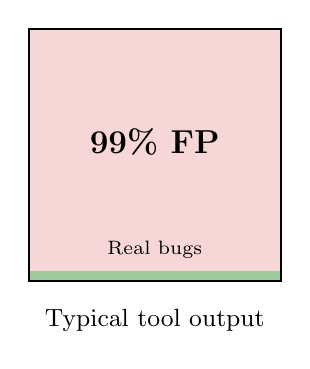
\begin{tikzpicture}[scale=0.8]
  \fill[msred!20] (0,0) rectangle (4,4);
  \fill[msgreen!40] (0,0) rectangle (4,0.15);
  \node at (2,2.2) {\large\textbf{99\% FP}};
  \node at (2,0.5) {\scriptsize Real bugs};
  \draw[thick] (0,0) rectangle (4,4);
  \node[below] at (2,-0.3) {\small Typical tool output};
\end{tikzpicture}
\end{column}
\end{columns}

\end{frame}

% =============================================================
% SLIDE 3: A3's Approach (Big Picture)
% =============================================================
\begin{frame}{A3's Approach: Two-Phase Architecture}

\begin{center}
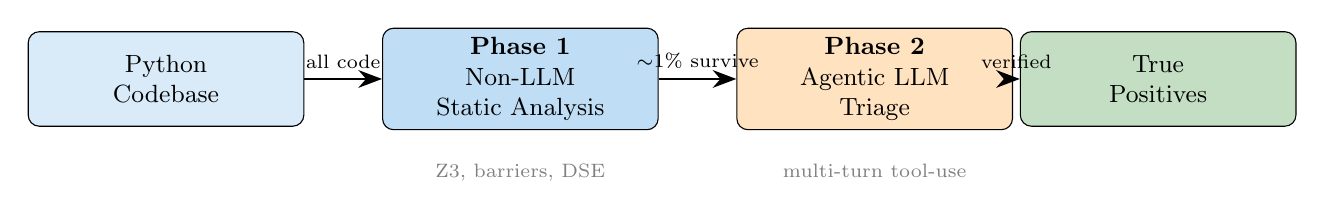
\begin{tikzpicture}[
  box/.style={draw, rounded corners, minimum width=3.5cm, minimum height=1.2cm, align=center, font=\small},
  arr/.style={-{Stealth[length=3mm]}, thick},
  scale=0.9
]
  \node[box, fill=msblue!15] (input) at (0,0) {Python\\Codebase};
  \node[box, fill=msblue!25] (phase1) at (5,0) {\textbf{Phase 1}\\Non-LLM\\Static Analysis};
  \node[box, fill=msorange!25] (phase2) at (10,0) {\textbf{Phase 2}\\Agentic LLM\\Triage};
  \node[box, fill=msgreen!25] (output) at (14,0) {True\\Positives};

  \draw[arr] (input) -- (phase1) node[midway,above,font=\scriptsize] {all code};
  \draw[arr] (phase1) -- (phase2) node[midway,above,font=\scriptsize] {$\sim$1\% survive};
  \draw[arr] (phase2) -- (output) node[midway,above,font=\scriptsize] {verified};

  \node[below=0.3cm of phase1, font=\scriptsize, text=gray] {Z3, barriers, DSE};
  \node[below=0.3cm of phase2, font=\scriptsize, text=gray] {multi-turn tool-use};
\end{tikzpicture}
\end{center}

\vspace{0.5em}
\begin{itemize}
  \item \textbf{Phase 1:} Formal methods filter the majority of false positives automatically
  \item \textbf{Phase 2:} An LLM agent \emph{explores the codebase} to classify survivors
  \item \textbf{Result:} High precision --- dramatically reduced noise
\end{itemize}

\end{frame}

% =============================================================
% Code Architecture
% =============================================================
\begin{frame}[fragile]{Codebase Architecture}

\begin{columns}[T]
\begin{column}{0.45\textwidth}
\begin{lstlisting}[style=bash,basicstyle=\ttfamily\tiny]
a3_python/
  cli.py          # CLI entry point
  analyzer.py     # Core engine
  frontend/       # Bytecode loading
  cfg/            # CFG + call graph
  semantics/      # Crash summaries
  z3model/        # Z3 value/heap
  unsafe/         # Bug predicates
  contracts/      # Taint src/sink
  dse/            # Concolic exec
  barriers/       # Certificate synth
  ci/             # CI integration
    sarif.py      # SARIF output
    baseline.py   # Ratchet
    agentic_triage.py
    templates/    # GH Actions
\end{lstlisting}
\end{column}
\begin{column}{0.52\textwidth}
\textbf{Dependencies:}
\begin{itemize}\setlength\itemsep{1pt}
  \item Core: \texttt{z3-solver} only
  \item CI: \texttt{+ anthropic, openai, pyyaml}
  \item Python $\geq$ 3.11 (bytecode format)
\end{itemize}
\vspace{0.5em}
\textbf{Design principles:}
\begin{itemize}\setlength\itemsep{1pt}
  \item Zero mandatory LLM dependency
  \item Formal methods first, LLM second
  \item SARIF as interchange format
  \item Modular: each \texttt{barriers/*.py} is an independent proof strategy
\end{itemize}
\end{column}
\end{columns}

\end{frame}

% =============================================================
% Phase 1 Pipeline
% =============================================================
\begin{frame}{Phase 1: The 7-Step Symbolic Execution Pipeline}

\begin{enumerate}
  \item \textbf{Call Graph Construction} --- whole-program CG from all \texttt{.py} files
  \item \textbf{Crash Summary Computation} --- bytecode disassembly $\to$ preconditions $\Pi_f$, effects $E_f$, exception sets $X_f$, nullability $N_f$
  \item \textbf{Symbolic Model Construction} --- Z3 representations: tagged values, heap model, taint lattice
  \item \textbf{Guard Detection} --- symbolic constraint extraction from \texttt{if}/\texttt{try}/\texttt{assert}/\texttt{isinstance}
  \item \textbf{Z3 Symbolic Execution} --- path feasibility via SMT satisfiability
  \item \textbf{Staged Portfolio (``Kitchensink'')} --- barrier certificates, $k$-induction, interpolation, IC3/PDR, CEGIS \emph{in parallel}
  \item \textbf{Classification} --- separate production code from test code
\end{enumerate}

\vspace{0.5em}
\textbf{Key:} Steps 4--6 are the formal-methods core.

\end{frame}

% =============================================================
% SLIDE 5: Call Graph & Bytecode Frontend
% =============================================================
\begin{frame}[fragile]{Step 1--2: Bytecode Frontend \& Call Graph}

\textbf{Frontend:} Uses Python's built-in \texttt{compile()} $\to$ \texttt{types.CodeType}
\begin{itemize}
  \item Disassembles bytecode instructions (CPython 3.11+)
  \item No AST heuristics --- operates on the \emph{actual} compiled representation
\end{itemize}

\vspace{0.5em}
\textbf{Call Graph:} $G_{\text{call}} = (V, E)$
\begin{itemize}
  \item $V$ = all functions (from bytecode \texttt{co\_consts})
  \item $E$ = call edges from \texttt{CALL} / \texttt{CALL\_FUNCTION} instructions
\end{itemize}

\vspace{0.5em}
\textbf{CFG per function:}
\begin{itemize}
  \item \texttt{BasicBlock}: id, offsets, instructions, successors
  \item Edge types: \texttt{FALLTHROUGH}, \texttt{JUMP}, \texttt{COND\_TRUE}, \texttt{COND\_FALSE}, \texttt{EXCEPTION}
  \item Exception regions with handler locations and nesting depth
\end{itemize}

\end{frame}

% =============================================================
% SLIDE 6: Barrier Certificates --- The Core Idea
% =============================================================
\begin{frame}{Barrier Certificates: Safety Without Exhaustive Search}

\textbf{Idea:} Construct a function $B : S \to \mathbb{R}$ that separates safe from unsafe states.

\begin{block}{Barrier Certificate Conditions}
\begin{align*}
  \textbf{Init:} \quad & \forall s_0 \in S_0.\; B(s_0) \geq \varepsilon \\
  \textbf{Inductive:} \quad & \forall s.\; B(s) \geq 0 \implies B(s') \geq 0 \\
  \textbf{Unsafe:} \quad & \forall s \in U.\; B(s) \leq -\varepsilon
\end{align*}
\end{block}

\textbf{If all three hold, the unsafe region is provably unreachable.}

\vspace{0.5em}
\begin{itemize}
  \item \textbf{Templates:} Linear, quadratic, polynomial, disjunctive regions
  \item \textbf{Synthesis:} Enumerate templates; validate with Z3; first inductive certificate wins
  \item \textbf{Specialized variants:} Hybrid (multi-mode), stochastic (supermartingale/It\^o), SOS, ranking functions
\end{itemize}

\end{frame}

% =============================================================
% SLIDE 7: Barrier Synthesis Algorithm
% =============================================================
\begin{frame}{Barrier Synthesis: Template Enumeration}

\textbf{11 template phases} (tried in increasing complexity):

\begin{columns}[T]
\begin{column}{0.48\textwidth}
\begin{enumerate}\setlength\itemsep{0pt}
  \item Constant barriers (trivial)
  \item Single-variable linear: $c_0 + c_1 x$
  \item Stack depth barriers
  \item Loop range barriers
  \item Collection size barriers
  \item Progress measures (termination)
\end{enumerate}
\end{column}
\begin{column}{0.48\textwidth}
\begin{enumerate}\setlength\itemsep{0pt}\setcounter{enumi}{6}
  \item Two-variable linear: $c_0 + c_1 v_1 + c_2 v_2$
  \item Quadratic: $ax^2 + bx + c$
  \item Bivariate quadratic: $x^2 + y^2 \leq R^2$
  \item Cubic polynomials
  \item Piecewise / disjunctive regions
\end{enumerate}
\end{column}
\end{columns}

\vspace{0.5em}
\textbf{Algorithm:}
\begin{enumerate}
  \item For each template $T_i$ in order of complexity:
  \item Instantiate $B = T_i$ with symbolic coefficients $\vec{c}$
  \item Encode Init $\land$ Inductive $\land$ Unsafe conditions as Z3 assertions
  \item If SAT: extract $\vec{c}$ $\Rightarrow$ \textbf{certificate found}, stop
  \item If UNSAT or timeout: try next template
\end{enumerate}

\end{frame}

% =============================================================
% SLIDE 8: Guard-to-Barrier Translation
% =============================================================
\begin{frame}{Guard-to-Barrier: From Code Patterns to Proofs}

\textbf{Key insight:} User guards in code map directly to barrier certificates.

\vspace{0.5em}
\begin{tabular}{lll}
\textbf{Guard Pattern} & \textbf{Barrier $B$} & \textbf{Bug Type} \\
\hline
\texttt{if x is not None} & $B(x) = (x \neq \texttt{None})\ ?\ 1 : {-}1$ & \texttt{NULL\_PTR} \\
\texttt{if xs} (truthiness) & $B(\texttt{xs}) = \texttt{len(xs)} - 1$ & \texttt{BOUNDS} \\
\texttt{if b != 0} & $B(b) = |b| - \varepsilon$ & \texttt{DIV\_ZERO} \\
\texttt{if k in d} & $B(k,d) = (k \in d)\ ?\ 1 : {-}1$ & \texttt{KEY\_ERROR} \\
\texttt{if i < len(xs)} & $B(i,\texttt{xs}) = (i \in [0, \texttt{len}))\ ?\ 1 : {-}1$ & \texttt{BOUNDS} \\
\end{tabular}

\vspace{0.5em}
\textbf{Validation:} Each translated barrier is checked for inductiveness by Z3.\\
\textbf{Advantage:} Replaces ad-hoc pattern matching with formal proofs.

\end{frame}

% =============================================================
% SLIDE 9: Z3 Symbolic Model
% =============================================================
\begin{frame}{Z3 Symbolic Model of Python Values}

\textbf{Tagged symbolic values:} \texttt{SymbolicValue(tag, payload, taint)}

\begin{columns}[T]
\begin{column}{0.5\textwidth}
\textbf{Value tags:}
\begin{itemize}
  \item \texttt{NONE, BOOL, INT, FLOAT}
  \item \texttt{STR, LIST, TUPLE, DICT}
  \item \texttt{OBJ, SLICE, ELLIPSIS}
\end{itemize}
\vspace{0.3em}
\textbf{Payload:} Z3 \texttt{IntSort}/\texttt{RealSort}/\texttt{ObjId}
\end{column}
\begin{column}{0.5\textwidth}
\textbf{Heap model:}
\begin{itemize}
  \item \texttt{SeqLen(obj\_id)} --- Z3 function
  \item \texttt{HasKey(dict\_id, key)} --- Z3 function
  \item \texttt{DictSize(obj\_id)} --- Z3 function
  \item Sequence: length + element map
  \item Taint lattice per value
\end{itemize}
\end{column}
\end{columns}

\vspace{0.5em}
\textbf{Example constraint:}
\[
  \texttt{tag} = \texttt{LIST} \;\land\; \texttt{SeqLen(id)} \geq 0 \;\land\; \texttt{idx} < \texttt{SeqLen(id)} \implies \text{BOUNDS safe}
\]

\end{frame}

% =============================================================
% SLIDE 7: Guard Detection
% =============================================================
\begin{frame}[fragile]{Guard Detection: Proving Bugs Unreachable}

A3 recognizes when bugs are already guarded in user code:

\begin{lstlisting}
def safe_divide(a, b):
    if b != 0:               # guard: b != 0
        return a / b          # DIV_ZERO unreachable!
    return 0.0
\end{lstlisting}

\textbf{Symbolic reasoning:}
\begin{enumerate}
  \item Extract guard constraint: $b \neq 0$
  \item Bug condition: $b = 0$
  \item Check SAT($b \neq 0 \;\land\; b = 0$) $= \text{UNSAT}$
  \item $\Rightarrow$ Proven false positive
\end{enumerate}

\vspace{0.3em}
\textbf{Detected guard patterns:}
\texttt{if x is not None} $\cdot$
\texttt{if xs} (truthiness) $\cdot$
\texttt{if b != 0} $\cdot$
\texttt{if k in d} $\cdot$
\texttt{if i < len(xs)}

\end{frame}

% =============================================================
% SLIDE 12: Directed Symbolic Execution (DSE)
% =============================================================
\begin{frame}{Directed Symbolic Execution (DSE)}

\textbf{Goal:} Confirm or refute bug reachability via constraint solving.

\vspace{0.5em}
\textbf{Algorithm:}
\begin{enumerate}
  \item Enumerate paths through the CFG to the bug location
  \item For each path, accumulate a \textbf{path condition} $\text{PC} = \bigwedge_i g_i$
  \item Conjoin the \textbf{bug condition} $\phi_{\text{bug}}$
  \item Query Z3: SAT($\text{PC} \land \phi_{\text{bug}}$)?
\end{enumerate}

\vspace{0.5em}
\begin{columns}[T]
\begin{column}{0.48\textwidth}
\textbf{If SAT:}
\begin{itemize}
  \item Extract concrete inputs from Z3 model
  \item \textbf{DSE-confirmed true positive}
  \item Provides a \emph{witness} (counterexample)
\end{itemize}
\end{column}
\begin{column}{0.48\textwidth}
\textbf{If UNSAT:}
\begin{itemize}
  \item Bug is \textbf{provably unreachable}
  \item Classified as false positive
  \item No further investigation needed
\end{itemize}
\end{column}
\end{columns}

\vspace{0.3em}
\textbf{Key data structure:} \texttt{DSEResult} (status: realized$|$failed$|$error), with concrete inputs from Z3 model

\end{frame}

% =============================================================
% SLIDE 13: Taint Analysis
% =============================================================
\begin{frame}{Taint Analysis for Security Bugs}

\textbf{Taint lattice:} Each \texttt{SymbolicValue} carries a set of taint labels.

\vspace{0.3em}
\begin{columns}[T]
\begin{column}{0.48\textwidth}
\textbf{Registered taint sources} ($\tau = 1$):
\begin{itemize}\setlength\itemsep{0pt}
  \item HTTP: \texttt{request.args}, \texttt{request.GET}
  \item User: \texttt{input()}, \texttt{sys.stdin}
  \item Env: \texttt{os.environ}, \texttt{os.getenv}
  \item Network: \texttt{urllib}, \texttt{requests}
  \item DB: \texttt{cursor.fetchone/all}
\end{itemize}
\end{column}
\begin{column}{0.48\textwidth}
\textbf{Registered taint sinks}:
\begin{itemize}\setlength\itemsep{0pt}
  \item \texttt{cursor.execute} $\to$ SQL\_INJECTION
  \item \texttt{os.system/popen} $\to$ CMD\_INJECTION
  \item \texttt{eval()/exec()} $\to$ CODE\_INJECTION
  \item \texttt{pickle.loads} $\to$ UNSAFE\_DESER
  \item HTML render $\to$ XSS
\end{itemize}
\end{column}
\end{columns}

\vspace{0.5em}
\textbf{Status:} Source/sink contracts and unsafe predicates are registered (48 security types). Taint propagation through the symbolic execution engine is a work in progress --- currently, correctness bugs (NULL\_PTR, DIV\_ZERO, BOUNDS) are the primary detection targets.

\end{frame}

% =============================================================
% SLIDE 14: Crash Summaries (Interprocedural)
% =============================================================
\begin{frame}{Interprocedural Analysis via Crash Summaries}

\textbf{Each function gets a \texttt{CrashSummary}:}

\begin{tabular}{ll}
  $\Pi_f$ (\texttt{preconditions})  & Required parameter conditions (non-None, typed, bounded) \\
  $E_f$ (\texttt{may\_trigger})     & Bug types function may trigger (+ \texttt{transitive\_bugs}) \\
  $X_f$ (\texttt{may\_raise})       & Exception types that may propagate \\
  $N_f$ (\texttt{param\_nullability}) & Which params/returns may be \texttt{None} \\
\end{tabular}

\vspace{0.5em}
\textbf{Interprocedural propagation:}
\begin{itemize}
  \item Caller passes value violating callee's $\Pi_f$ $\Rightarrow$ potential \texttt{NULL\_PTR}
  \item Uncaught exception in $X_f$ $\Rightarrow$ propagates to caller
  \item Guard in caller can satisfy callee's $\Pi_f$ $\Rightarrow$ eliminates $E_f$
\end{itemize}

\end{frame}

% =============================================================
% SLIDE 9: Bug Types Detected
% =============================================================
\begin{frame}{84 Bug Types Across Correctness \& Security}

\begin{columns}[T]
\begin{column}{0.48\textwidth}
\textbf{Correctness (36 types):}
\begin{itemize}\setlength\itemsep{0pt}
  \item \texttt{DIV\_ZERO}, \texttt{NULL\_PTR}, \texttt{BOUNDS}
  \item \texttt{ASSERT\_FAIL}, \texttt{UNBOUND\_LOCAL}
  \item \texttt{INTEGER\_OVERFLOW}, \texttt{FP\_DOMAIN}
  \item \texttt{VALUE\_ERROR}, \texttt{RUNTIME\_ERROR}
  \item \texttt{NON\_TERMINATION}, \texttt{STACK\_OVERFLOW}
  \item \texttt{MEMORY\_LEAK}, \texttt{USE\_AFTER\_FREE}
  \item \texttt{DATA\_RACE}, \texttt{DEADLOCK}
  \item \texttt{TYPE\_CONFUSION}, \texttt{NAME\_ERROR}
  \item + 19 more (IO, file, module, etc.)
\end{itemize}
\end{column}
\begin{column}{0.48\textwidth}
\textbf{Security (48 types):}
\begin{itemize}\setlength\itemsep{0pt}
  \item \textbf{Injection:} SQL, Command, Code, Path, LDAP, XPath, NoSQL, Regex, Header, Cookie, Log
  \item \textbf{Web:} XSS, SSRF, CSRF, URL redirect
  \item \textbf{Crypto:} Weak crypto/key, broken algorithm, insecure protocol
  \item \textbf{Deser:} Pickle/YAML/XML unsafe loads, XXE
  \item \textbf{Secrets:} Cleartext logging/storage, hardcoded creds
  \item \textbf{ReDoS:} Polynomial/exponential regex
\end{itemize}
\end{column}
\end{columns}

\vspace{0.3em}
Each type has a registered \textbf{unsafe predicate} and \textbf{barrier template} for synthesis.

\end{frame}

% =============================================================
% Unsafe Predicates: How Bugs Are Defined
% =============================================================
\begin{frame}[fragile]{Unsafe Predicates: Formal Bug Definitions}

Each bug type is defined by a \textbf{predicate} on the symbolic state:

\vspace{0.3em}
\textbf{Registry:} \texttt{UNSAFE\_PREDICATES: dict[bug\_type $\to$ (predicate, extractor)]}

\vspace{0.3em}
\begin{tabular}{lll}
\textbf{Bug Type} & \textbf{Predicate $P(\sigma)$} & \textbf{Extractor} \\
\hline
\texttt{DIV\_ZERO} & $\texttt{divisor}(\sigma) = 0$ & divisor value \\
\texttt{NULL\_PTR} & $\texttt{tag}(\sigma.v) = \texttt{NONE} \;\land\; \texttt{deref}(\sigma)$ & variable name \\
\texttt{BOUNDS} & $\texttt{idx}(\sigma) \geq \texttt{SeqLen}(\sigma.s)$ & index, length \\
\texttt{SQL\_INJ} & $\tau(\sigma.q) = 1 \;\land\; \lnot\texttt{Param}(\sigma)$ & tainted query \\
\texttt{CMD\_INJ} & $\tau(\sigma.\text{arg}) = 1 \;\land\; \texttt{at\_shell\_sink}$ & command string \\
\end{tabular}

\vspace{0.5em}
\textbf{Four predicate categories:}
\begin{enumerate}\setlength\itemsep{0pt}
  \item \textbf{Correctness} (36): DIV\_ZERO, NULL\_PTR, BOUNDS, etc.
  \item \textbf{Security} (48): injection, crypto, deser, secrets, ReDoS
\end{enumerate}

\end{frame}

% =============================================================
% Phase 2 --- Agentic Triage
% =============================================================
\begin{frame}{Phase 2: Agentic LLM Triage}

For findings that survive formal verification:

\begin{center}
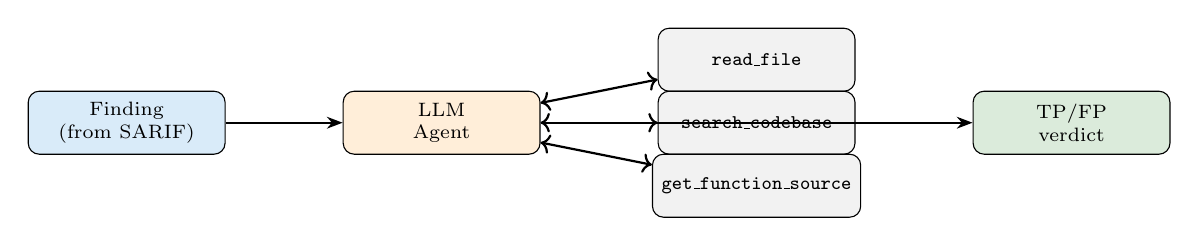
\begin{tikzpicture}[
  box/.style={draw, rounded corners, minimum width=2.5cm, minimum height=0.8cm, align=center, font=\scriptsize},
  arr/.style={-{Stealth[length=2mm]}, thick},
]
  \node[box, fill=msblue!15] (finding) at (0,0) {Finding\\(from SARIF)};
  \node[box, fill=msorange!15] (llm) at (4,0) {LLM\\Agent};
  \node[box, fill=gray!10] (tools) at (8,0.8) {\texttt{read\_file}};
  \node[box, fill=gray!10] (tools2) at (8,0) {\texttt{search\_codebase}};
  \node[box, fill=gray!10] (tools3) at (8,-0.8) {\texttt{get\_function\_source}};
  \node[box, fill=msgreen!15] (verdict) at (12,0) {TP/FP\\verdict};

  \draw[arr] (finding) -- (llm);
  \draw[arr,<->] (llm) -- (tools);
  \draw[arr,<->] (llm) -- (tools2);
  \draw[arr,<->] (llm) -- (tools3);
  \draw[arr] (llm) -- (verdict);
\end{tikzpicture}
\end{center}

\textbf{Tools available:} \texttt{read\_file}, \texttt{search\_codebase}, \texttt{get\_function\_source}, \texttt{get\_imports}, \texttt{list\_directory}, \texttt{classify}

\vspace{0.3em}
\begin{itemize}
  \item \textbf{Not a one-shot prompt} --- multi-turn, iterative investigation (2--6 tool calls)
  \item Agent reads callers, checks tests, follows imports, verifies guards
  \item Calls \texttt{classify(verdict, confidence, rationale)} when ready
\end{itemize}

\end{frame}

% =============================================================
% SLIDE 11: Verdicts & Confidence
% =============================================================
\begin{frame}{Three Verdicts}

\begin{center}
\begin{tabular}{lll}
\textbf{Verdict} & \textbf{Meaning} & \textbf{Fraction} \\
\hline
\textcolor{msgreen}{\textbf{FP (proven)}} & Barrier certificate or DSE proves unreachability & majority \\
\textcolor{msorange}{\textbf{TP candidate}} & No proof found; sent to LLM triage & remainder \\
\textcolor{msred}{\textbf{DSE-confirmed TP}} & Z3 found satisfying input triggering the crash & rare \\
\end{tabular}
\end{center}

\vspace{1em}
\textbf{Confidence scoring:}
\begin{itemize}
  \item Each finding gets a confidence score $c \in [0, 1]$
  \item Barrier proof $\Rightarrow c$ reduced toward 0 (FP)
  \item DSE witness $\Rightarrow c$ increased toward 1 (TP)
  \item LLM agent provides independent confidence + rationale
\end{itemize}

\end{frame}

% =============================================================
% Agentic Conversation: How the Agent Investigates
% =============================================================
\begin{frame}[fragile]{Agentic Investigation: A Concrete Trace}

\textbf{Finding:} \texttt{NULL\_PTR} in \texttt{get\_user\_email()} at line 42

\vspace{0.3em}
\begin{tabular}{rp{11cm}}
\textbf{Turn 1:} & Agent receives finding + function source \\
\textbf{Turn 2:} & \texttt{search\_codebase("get\_user\_email")} --- finds 3 callers \\
\textbf{Turn 3:} & \texttt{read\_file("views.py", 100, 120)} --- caller checks \texttt{if user:} \\
\textbf{Turn 4:} & \texttt{get\_function\_source("validate\_user")} --- confirms None check \\
\textbf{Turn 5:} & \texttt{classify(verdict="FP", confidence=0.9,}\\
                 & \texttt{rationale="All callers guard against None")} \\
\end{tabular}

\vspace{0.5em}
\textbf{Key design decisions:}
\begin{itemize}
  \item Max \textbf{10 turns} per finding (Turn 9: ``call \texttt{classify} NOW'')
  \item Tool output truncated to \textbf{6000 chars}
  \item Uses OpenAI function-calling format (converted for Anthropic)
  \item Providers: GitHub Models (free), OpenAI, Anthropic
\end{itemize}

\end{frame}

% =============================================================
% Scripted Example 1 --- NULL_PTR
% =============================================================
\begin{frame}[fragile]{Demo 1: NULL\_PTR Detection \& Guard Elimination}

\begin{columns}[T]
\begin{column}{0.48\textwidth}
\textbf{Unsafe version:}
\begin{lstlisting}
def authenticate(username, db):
    record = db.get(username)
    # record could be None!
    return record['password_hash']
    # => NULL_PTR reported
\end{lstlisting}
\vspace{0.5em}
\begin{lstlisting}[style=bash]
$ a3 scan unsafe.py
NULL_PTR: authenticate
  unsafe.py:1  Confidence: 0.76
Total bugs found: 1
\end{lstlisting}
\end{column}
\begin{column}{0.48\textwidth}
\textbf{Safe version:}
\begin{lstlisting}
def authenticate(username, db):
    record = db.get(username)
    if record is not None:
        return record['password_hash']
    return None
\end{lstlisting}
\vspace{0.5em}
\begin{lstlisting}[style=bash]
$ a3 scan safe.py
Total bugs found: 0
\end{lstlisting}
\vspace{0.3em}
\textcolor{msgreen}{\textbf{Z3:}} SAT($\texttt{record} \neq \texttt{None} \;\land\; \texttt{record} = \texttt{None}$) = UNSAT $\checkmark$
\end{column}
\end{columns}

\end{frame}

% =============================================================
% SLIDE 13: Scripted Example 2 --- DIV_ZERO
% =============================================================
\begin{frame}[fragile]{Demo 2: DIV\_ZERO with Guard Detection}

\begin{lstlisting}
def ratio(a, b):
    return a / b   # DIV_ZERO: b could be 0
\end{lstlisting}

\begin{lstlisting}[style=bash]
$ a3 scan ratio.py
DIV_ZERO: ratio
  ratio.py:1    Confidence: 0.84
Total bugs found: 1
\end{lstlisting}

\vspace{0.3em}
\textbf{Now add a guard:}
\begin{lstlisting}
def ratio(a, b):
    if b != 0:
        return a / b   # Now proven safe
    return 0.0
\end{lstlisting}

\begin{lstlisting}[style=bash]
$ a3 scan ratio_safe.py
Total bugs found: 0
\end{lstlisting}

\textbf{Z3 reasoning:} Guard $b \neq 0$ makes bug condition $b = 0$ unsatisfiable at division site.

\end{frame}

% =============================================================
% SLIDE 14: Scripted Example 3 --- SQL Injection
% =============================================================
\begin{frame}[fragile]{Demo 3: NULL\_PTR --- Chained Attribute Access}

\begin{columns}[T]
\begin{column}{0.48\textwidth}
\textbf{Unsafe:}
\begin{lstlisting}
def get_host(config):
    return config.database.host
    # NULL_PTR: config or
    # config.database could be None
\end{lstlisting}

\begin{lstlisting}[style=bash]
$ a3 scan app.py
NULL_PTR: get_host
  app.py:1  Confidence: 0.76
Total bugs found: 1
\end{lstlisting}
\end{column}
\begin{column}{0.48\textwidth}
\textbf{Safe:}
\begin{lstlisting}
def get_host(config):
    if config is not None \
       and config.database is not None:
        return config.database.host
    return "localhost"
\end{lstlisting}

\begin{lstlisting}[style=bash]
$ a3 scan app_safe.py
Total bugs found: 0
\end{lstlisting}
\vspace{0.3em}
\textcolor{msgreen}{\textbf{Guard detected:}} None-checks eliminate NULL\_PTR at each dereference.
\end{column}
\end{columns}

\end{frame}

% =============================================================
% SLIDE 15: Scripted Example 4 --- BOUNDS + Interprocedural
% =============================================================
\begin{frame}[fragile]{Demo 4: Multiple Bug Types in One Function}

\begin{lstlisting}
def process_record(records, index, divisor):
    record = records[index]            # BOUNDS
    value = record['amount'] / divisor # DIV_ZERO
    return value
\end{lstlisting}

\begin{lstlisting}[style=bash]
$ a3 scan example.py
BOUNDS: process_record    example.py:1    Confidence: 0.76
DIV_ZERO: process_record  example.py:1    Confidence: 0.84
Total bugs found: 2
\end{lstlisting}

\vspace{0.3em}
\textbf{Add guards for both:}
\begin{lstlisting}
def process_record(records, index, divisor):
    if records and index < len(records) and divisor != 0:
        record = records[index]
        value = record['amount'] / divisor
        return value
    return None
\end{lstlisting}
\vspace{-0.3em}
\begin{lstlisting}[style=bash]
$ a3 scan example_safe.py
Total bugs found: 0
\end{lstlisting}

\end{frame}

% =============================================================
% Demo 5: Unsafe Deserialization
% =============================================================
\begin{frame}[fragile]{Demo 5: BOUNDS --- Truthiness Guard}

\begin{columns}[T]
\begin{column}{0.48\textwidth}
\textbf{Unsafe:}
\begin{lstlisting}
def first_element(items):
    return items[0]
    # BOUNDS: items could be empty
\end{lstlisting}

\begin{lstlisting}[style=bash]
$ a3 scan head.py --min-confidence 0
BOUNDS: first_element
  head.py:1  Confidence: 0.53
Total bugs found: 1
\end{lstlisting}
\end{column}
\begin{column}{0.48\textwidth}
\textbf{Safe:}
\begin{lstlisting}
def first_element(items):
    if items:
        return items[0]
    return None
\end{lstlisting}

\begin{lstlisting}[style=bash]
$ a3 scan head_safe.py --min-confidence 0
Total bugs found: 0
\end{lstlisting}
\vspace{0.3em}
\textbf{Guard:} Python truthiness check (\texttt{if items}) detected as non-empty guard for list access.
\end{column}
\end{columns}

\end{frame}

% =============================================================
% Demo 6: Command Injection
% =============================================================
\begin{frame}[fragile]{Demo 6: DIV\_ZERO --- Truthiness vs Explicit Guard}

\begin{lstlisting}
def calculate_average(scores):
    total = sum(scores)
    return total / len(scores)   # DIV_ZERO if scores is empty
\end{lstlisting}

\begin{lstlisting}[style=bash]
$ a3 scan avg.py
DIV_ZERO: calculate_average   avg.py:1   Confidence: 0.84
Total bugs found: 1
\end{lstlisting}

\vspace{0.3em}
\textbf{Guard with truthiness check} (detected):
\begin{lstlisting}
def calculate_average(scores):
    if not scores:
        return 0.0
    return sum(scores) / len(scores)
\end{lstlisting}
\vspace{-0.3em}
\begin{lstlisting}[style=bash]
$ a3 scan avg_safe.py
Total bugs found: 0
\end{lstlisting}

\textbf{Note:} \texttt{if not scores} is detected as a guard; \texttt{if len(scores) == 0} currently is not (direct \texttt{len()} comparison is a known gap).

\end{frame}

% =============================================================
% Proof Strategies Portfolio
% =============================================================
\begin{frame}{Proof Strategy Portfolio (``Kitchensink'')}

Multiple verification techniques run \textbf{in parallel} --- first proof wins:

\vspace{0.5em}
\begin{tabular}{lll}
\textbf{Strategy} & \textbf{Strength} & \textbf{Reference} \\
\hline
Barrier certificates & Continuous safety & Prajna \& Jadbabaie, 2004 \\
$k$-induction & Bounded loops & Sheeran et al., 2000 \\
IC3/PDR & Property-directed & Bradley, 2011 \\
Craig interpolation & Refinement & McMillan, 2003 \\
CEGIS & Synthesis & Solar-Lezama, 2008 \\
SOS (Positivstellensatz) & Polynomial & Parrilo, 2003 \\
Ranking functions & Termination & Cook et al., 2006 \\
Houdini & Annotation inference & Flanagan \& Leino, 2001 \\
\end{tabular}

\vspace{0.5em}
\textbf{Why portfolio?} Different proof strategies excel on different code patterns.\\
Running them in parallel gives best coverage without strategy selection.

\end{frame}

% =============================================================
% SLIDE 17: CI Integration
% =============================================================
\begin{frame}[fragile]{Zero-Config CI Integration}

\begin{lstlisting}[style=bash]
$ a3 init . --copilot
$ git add .github/ .a3.yml .a3-baseline.json
$ git push
\end{lstlisting}

\vspace{0.5em}
\textbf{What happens on every push/PR:}
\begin{enumerate}
  \item Non-LLM scan $\to$ SARIF
  \item Agentic triage (uses \texttt{GITHUB\_TOKEN} --- free, zero config)
  \item Baseline ratchet check (new bugs $\Rightarrow$ CI fails)
  \item SARIF uploaded to GitHub Code Scanning dashboard
\end{enumerate}

\vspace{0.5em}
\textbf{Baseline ratchet} for incremental adoption:
\begin{itemize}
  \item New findings not in baseline $\Rightarrow$ \textcolor{msred}{CI fails}
  \item Findings that disappear $\Rightarrow$ auto-pruned
  \item Pre-existing issues $\Rightarrow$ ignored (never blocked on legacy debt)
\end{itemize}

\end{frame}

% =============================================================
% Formal Semantics: What Is Modeled
% =============================================================
\begin{frame}{Formal Semantics: The Python Subset}

\textbf{What A3 models:}
\begin{itemize}
  \item \textbf{Values:} \texttt{None}, booleans, integers (unbounded), floats, strings (length-abstracted)
  \item \textbf{Collections:} Lists, tuples, dicts --- modeled as $(\text{length}, \text{element\_map})$
  \item \textbf{Control flow:} \texttt{if/else}, \texttt{for/while}, \texttt{try/except/finally}, \texttt{with}
  \item \textbf{Functions:} First-class, closures, \texttt{*args}/\texttt{**kwargs}
  \item \textbf{Objects:} Attribute access, \texttt{isinstance}, method resolution
\end{itemize}

\vspace{0.5em}
\textbf{What A3 approximates:}
\begin{itemize}
  \item \textbf{Dynamic dispatch:} Over-approximated in call graph (all possible targets)
  \item \textbf{Heap aliasing:} ObjId-based, not full shape analysis
  \item \textbf{Strings:} Length-tracked; content analysis only for taint
  \item \textbf{Generators/async:} Treated as ordinary functions
\end{itemize}

\vspace{0.3em}
\textbf{Soundness guarantee:} Barrier proofs are sound \emph{for the modeled semantics}. The gap between model and CPython is the source of unsoundness.

\end{frame}

% =============================================================
% Evaluation: BugsInPy
% =============================================================
\begin{frame}{Evaluation on Real-World Python Projects}

\textbf{BugsInPy benchmark:} 493 real bugs from 17 large Python projects\\
(pandas, scikit-learn, flask, tornado, youtube-dl, black, \ldots)

\vspace{0.5em}
\begin{columns}[T]
\begin{column}{0.48\textwidth}
\textbf{Phase 1 (static analysis):}
\begin{itemize}
  \item Filters guarded bugs as FP
  \item Barrier certificates prove guards
  \item DSE confirms subset as TP
  \item Runs in seconds per file
\end{itemize}
\end{column}
\begin{column}{0.48\textwidth}
\textbf{Phase 2 (agentic triage):}
\begin{itemize}
  \item Classifies unproven findings
  \item 2--6 tool calls per finding
  \item Agent reads callers, tests, imports
  \item High precision on survivor set
\end{itemize}
\end{column}
\end{columns}

\vspace{0.5em}
\textbf{Key insight:} The two phases are \emph{complementary}:
\begin{itemize}
  \item Phase 1 eliminates what \emph{can} be proven formally
  \item Phase 2 handles the \emph{semantic ambiguity} that formal methods cannot resolve
\end{itemize}

\end{frame}

% =============================================================
% Soundness vs. Precision Tradeoff
% =============================================================
\begin{frame}{The Soundness--Precision Tradeoff}

\begin{center}
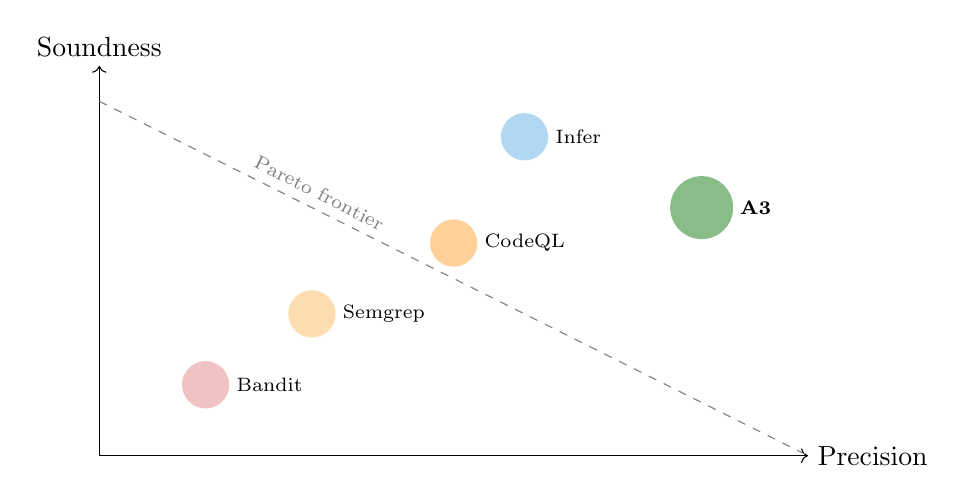
\begin{tikzpicture}[scale=0.9]
  \draw[->] (0,0) -- (10,0) node[right] {Precision};
  \draw[->] (0,0) -- (0,5.5) node[above] {Soundness};

  \node[circle, fill=msred!30, minimum size=0.6cm, font=\scriptsize] (bandit) at (1.5,1) {};
  \node[right, font=\scriptsize] at (1.8,1) {Bandit};

  \node[circle, fill=msorange!30, minimum size=0.6cm, font=\scriptsize] (semgrep) at (3,2) {};
  \node[right, font=\scriptsize] at (3.3,2) {Semgrep};

  \node[circle, fill=msorange!40, minimum size=0.6cm, font=\scriptsize] (codeql) at (5,3) {};
  \node[right, font=\scriptsize] at (5.3,3) {CodeQL};

  \node[circle, fill=msblue!30, minimum size=0.6cm, font=\scriptsize] (infer) at (6,4.5) {};
  \node[right, font=\scriptsize] at (6.3,4.5) {Infer};

  \node[circle, fill=msgreen!50, minimum size=0.8cm, font=\scriptsize\bfseries] (a3) at (8.5,3.5) {};
  \node[right, font=\scriptsize\bfseries] at (8.9,3.5) {A3};

  \draw[dashed, gray] (0,5) -- (10,0) node[pos=0.3, above, font=\scriptsize, text=gray, rotate=-27] {Pareto frontier};
\end{tikzpicture}
\end{center}

\vspace{0.3em}
\textbf{A3's position:} Sacrifices full soundness for \textbf{very high precision}.\\
Barrier proofs are locally sound; the LLM fallback handles the rest.\\
\textbf{Design principle:} A tool developers \emph{actually use} beats a sound tool they ignore.

\end{frame}

% =============================================================
% Formal Methods Questions
% =============================================================
\begin{frame}{Formal Methods FAQ (1/2)}

\textbf{Q: Is the analysis sound?}\\
A: \textbf{No.} Soundness is explicitly traded for precision. The barrier proofs are sound \emph{for the modeled semantics}, but the Python model is an approximation (no full heap semantics, dynamic dispatch is approximate).

\vspace{0.5em}
\textbf{Q: Is it complete?}\\
A: No. Template enumeration is incomplete; some safe programs lack polynomial barriers. The portfolio mitigates this but cannot guarantee completeness.

\vspace{0.5em}
\textbf{Q: What about dynamic features (eval, monkey-patching)?}\\
A: Conservatively flagged. Dynamic dispatch is over-approximated in the call graph. \texttt{eval}/\texttt{exec} are taint sinks (CODE\_INJECTION).

\vspace{0.5em}
\textbf{Q: How does it scale?}\\
A: Per-function analysis is linear in LOC. Interprocedural is bounded by call graph size. Z3 queries are typically small (10--100 constraints). Portfolio strategies have individual timeouts.

\end{frame}

% =============================================================
% Formal Methods FAQ (2/2)
% =============================================================
\begin{frame}{Formal Methods FAQ (2/2)}

\textbf{Q: Why barriers instead of abstract interpretation?}\\
A: Barriers provide \emph{per-bug} proofs (targeted) vs.\ whole-program invariants. Much cheaper for large codebases --- we only need to prove specific properties unreachable.

\vspace{0.5em}
\textbf{Q: How do you handle loops?}\\
A: Multiple strategies: $k$-induction for bounded loops, ranking functions for termination, barrier certificates for safety within loops. The portfolio tries all in parallel.

\vspace{0.5em}
\textbf{Q: What about the LLM --- isn't that unsound by definition?}\\
A: Yes. The LLM is \emph{not} part of the formal reasoning. It only classifies findings that \emph{already escaped} formal verification. Think of it as a high-quality human reviewer, not a proof engine.

\vspace{0.5em}
\textbf{Q: Can barrier proofs be checked independently?}\\
A: Yes. A barrier certificate is a \emph{witness}: given $B$, checking Init $\land$ Inductive $\land$ Unsafe is a Z3 query. Proof auditing is trivial compared to proof search.

\end{frame}

% =============================================================
% Open Problems for FM Community
% =============================================================
\begin{frame}{Open Problems for the FM Community}

\begin{enumerate}
  \item \textbf{Heap-sensitive barriers:} Can barrier certificates reason about linked structures, aliasing, and shape properties in Python?

  \item \textbf{Completeness of template enumeration:} What is the minimal template basis that covers ``common'' Python patterns? Is there a PAC-learning formulation?

  \item \textbf{Compositional taint proofs:} Can we compose per-function barrier certificates to get whole-program taint-freedom guarantees?

  \item \textbf{Certified Python semantics:} A mechanized (Lean/Coq) semantics of CPython 3.11+ bytecode would let us prove soundness of the Z3 model.

  \item \textbf{LLM-guided proof search:} Can an LLM suggest barrier templates or invariants that accelerate formal verification? (Neural certificate synthesis)

  \item \textbf{Incremental re-verification:} Given a diff, which barrier proofs are invalidated? Can we re-verify only affected functions?
\end{enumerate}

\end{frame}

% =============================================================
% Related Work & Positioning
% =============================================================
\begin{frame}{Related Work}

\begin{tabular}{llll}
\textbf{Tool} & \textbf{Approach} & \textbf{Precision} & \textbf{Formal?} \\
\hline
Bandit & Pattern matching & Low & No \\
Semgrep & Structural patterns & Medium & No \\
Pyright/mypy & Type checking & High (types only) & Partial \\
CodeQL & Dataflow queries & Medium-High & Partial \\
Infer & Separation logic & High & Yes \\
\textbf{A3} & \textbf{Barriers + DSE + LLM} & \textbf{Very High} & \textbf{Yes (Phase 1)} \\
\end{tabular}

\vspace{0.5em}
\textbf{Key differentiators:}
\begin{itemize}
  \item \textbf{Only Python-specific} barrier certificate tool
  \item \textbf{Portfolio of 8+ proof strategies} (not just one technique)
  \item \textbf{Agentic LLM fallback} for what formal methods can't prove
  \item \textbf{84 bug types} spanning correctness + security
\end{itemize}

\end{frame}

% =============================================================
% SLIDE 20: Future Directions & Questions
% =============================================================
\begin{frame}{Future Directions}

\begin{itemize}
  \item \textbf{Richer heap models:} Full shape analysis for Python containers
  \item \textbf{Neural barrier synthesis:} Learn barrier templates from code patterns
  \item \textbf{Incremental analysis:} Re-verify only changed functions on each commit
  \item \textbf{Cross-language:} Extend Z3 model to TypeScript/JavaScript
  \item \textbf{Formal soundness proofs:} Mechanize the Python subset semantics in Lean/Coq
\end{itemize}

\vspace{1em}
\begin{center}
\Large\textbf{Questions?}
\end{center}

\vspace{0.5em}
\begin{center}
\texttt{pip install a3-python} \quad|\quad \texttt{a3 scan . --triage}\\[0.3em]
\small\url{https://github.com/thehalleyyoung/a3-python}
\end{center}

\end{frame}

\end{document}
